%
% system_overview.tex
%
% Copyright (C) 2019 by SpaceLab.
%
% OBDH 2.0 Documentation
%
% This work is licensed under the Creative Commons Attribution-ShareAlike 4.0
% International License. To view a copy of this license,
% visit http://creativecommons.org/licenses/by-sa/4.0/.
%

%
% \brief System Overview chapter.
%
% \author Gabriel Mariano Marcelino <gabriel.mm8@gmail.com>
% \author André Martins Pio de Mattos <andrempmattos@gmail.com>
%
% \institution Universidade Federal de Santa Catarina (UFSC)
%
% \version 0.5.0
%
% \date 23/11/2019
%

\chapter{System Overview} \label{ch:system-overview}

The board has a MSP430 low-power microcontroller that runs the firmware application and several other peripherals for an extended operation and physical interfaces (i.e., non-volatile memory, watchdog timer, service modules and payloads interfaces, daughterboard interface, current monitor). The microcontroller manages the others sub-modules within the board using serial communication buses, synchronizes actions, handles communication with the ground segment, and manages the data flow. The programming language used is C and the firmware was developed using the Code Composer Studio IDE\nomenclature{\textbf{IDE}}{\textit{Integrated Development Environment.}} (a.k.a. CCS) for compiling, programming and testing. The module has many tasks, such as interfacing peripherals and other MCUs, over distinct protocols and time requirements. Then, in order to improve predictability, a Real Time Operating System (RTOS\nomenclature{\textbf{RTOS}}{\textit{Real Time Operating System.}}) is used to ensure that the deadlines are observed, even under a fault situation in a routine. The RTOS chosen is the FreeRTOS (v10.0.0), since it is designed for embedded systems applications and it was already validated in space applications. The firmware architecture follows an abstraction layer scheme to facilitate higher level implementations and allow more portability across different hardware platforms.

\section{Block Diagram}

The \autoref{fig:block-diagram} presents a simplified view of the module subsystems and interfaces. The microcontroller has a programming JTAG\nomenclature{\textbf{JTAG}}{\textit{Joint Test Action Group.}}
 and 6 communication buses, divided in 3 different protocols (I2C\nomenclature{\textbf{I2C}}{\textit{Inter-Integrated Circuit.}}, SPI\nomenclature{\textbf{SPI}}{\textit{Serial Peripheral Interface.}} and UART\nomenclature{\textbf{UART}}{\textit{Universal Asynchronous Receiver/Transmitter.}}), that are shared between all the peripherals and external interfaces. Besides this channels, there are GPIO\nomenclature{\textbf{GPIO}}{\textit{General Purpose Input/Output.}} connections for various functions, from control ports to status pins. There is a non-volatile memory device to store the satellite data frames and critical status indicators. There are buffers and transceivers intended to allow secure and proper communication with external modules. A watchdog timer with voltage monitor and a current sensor are attached to the system for improving the overall reliability and generating essential housekeeping data. There is a generic daughterboard interface for extending the module capabilities with an auxiliary application board. Also, directly connected to the microcontroller, there is a UART debug interface. More details and descriptions about these components and interfaces are provided in the \autoref{ch:hardware}.

\begin{figure}[!ht]
    \begin{center}
        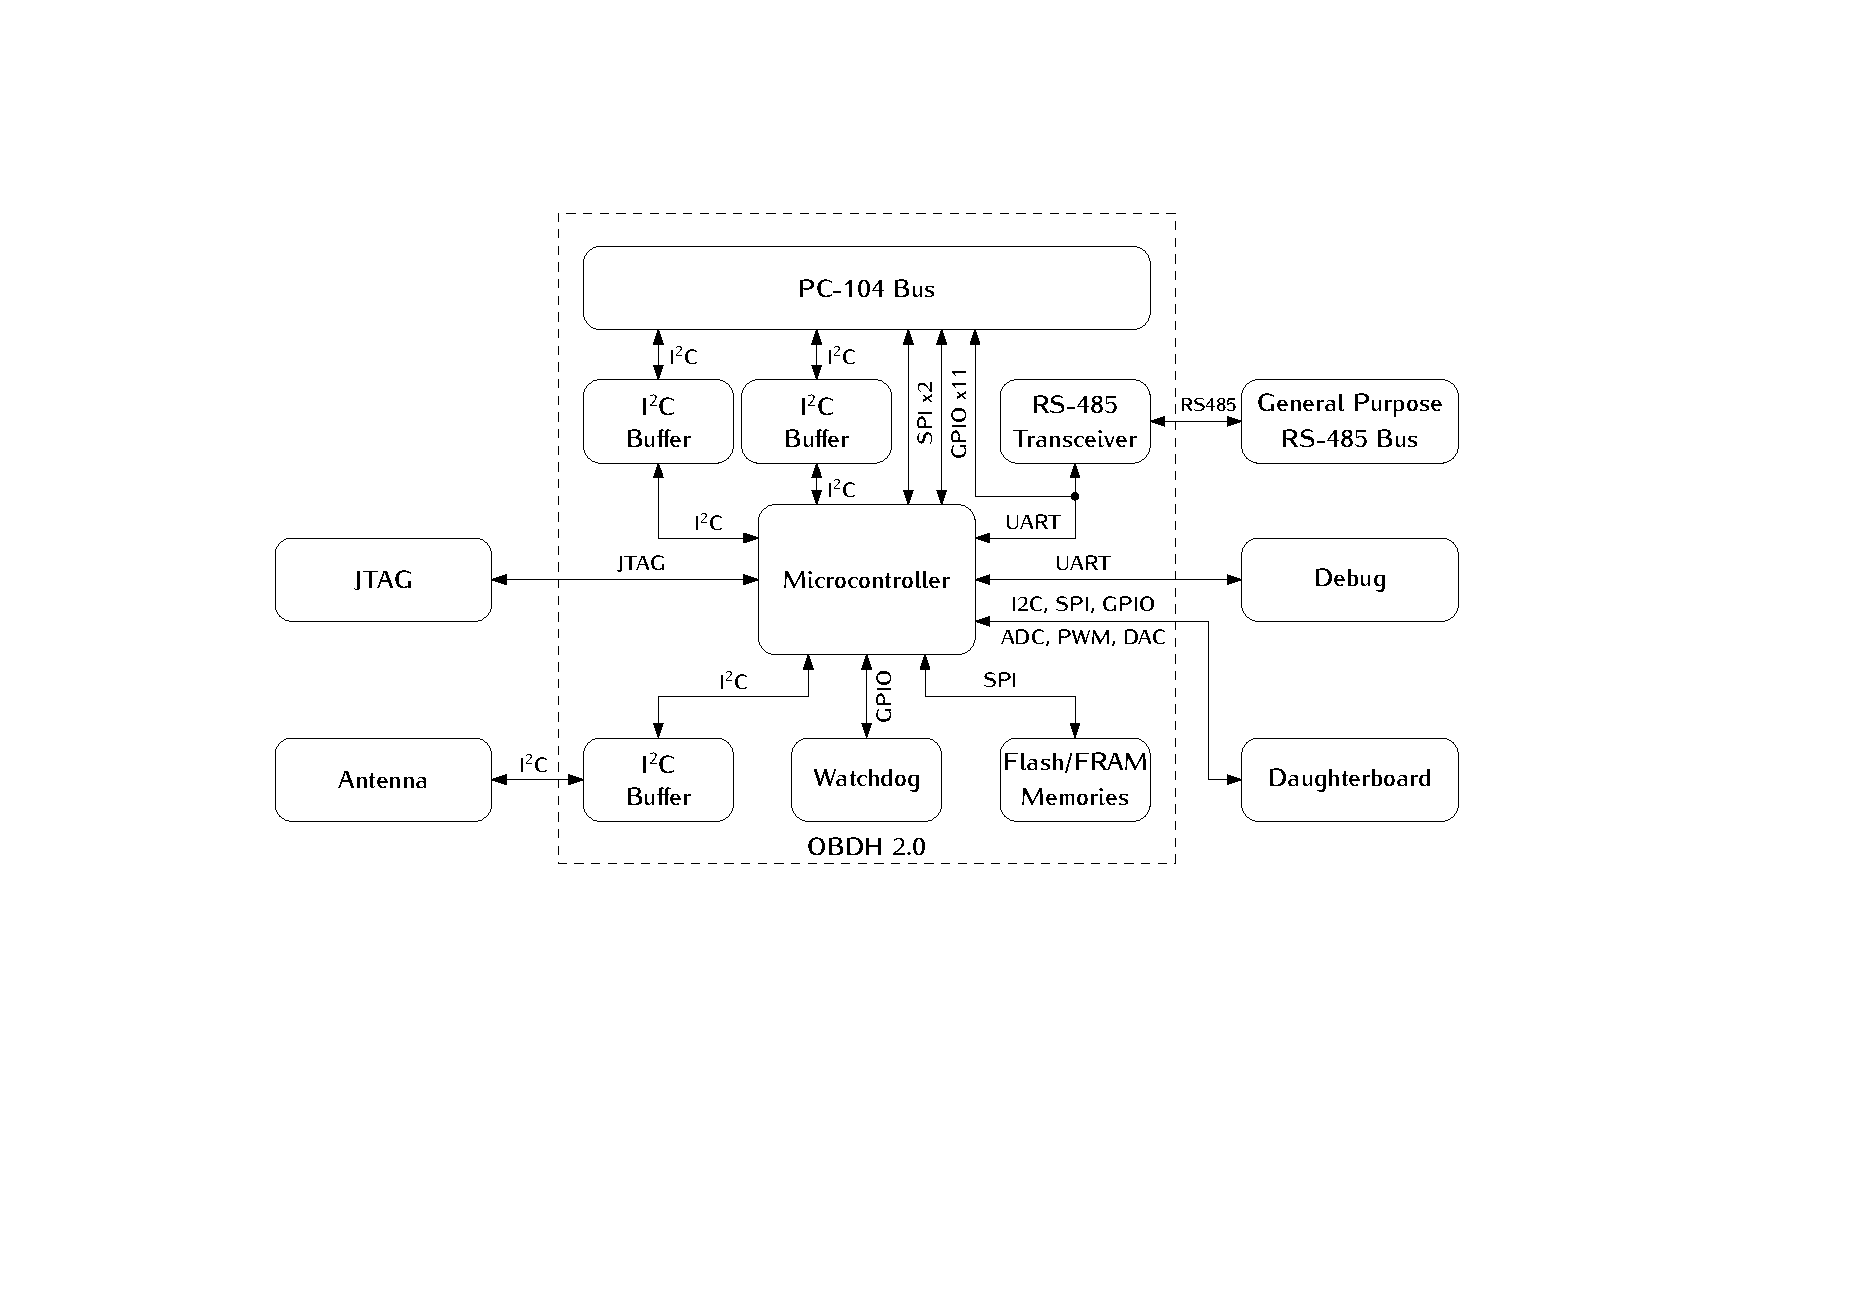
\includegraphics[width=\textwidth]{figures/block_diagram.pdf}
        \caption{OBDH 2.0 Block diagram.}
        \label{fig:block-diagram}
    \end{center}
\end{figure}

\section{System Layers}

As herein mentioned, the system is divided in various abstraction layers to favor high level firmware implementations. The \autoref{fig:system-layers} shows this scheme, which is composed of third-part drivers at the lowest layer above the hardware, the operating system as the base building block of the module, the devices handling implementation, and the application tasks in the highest layer. More details are provided in the \autoref{ch:firmware}.

\begin{figure}[!ht]
    \begin{center}
        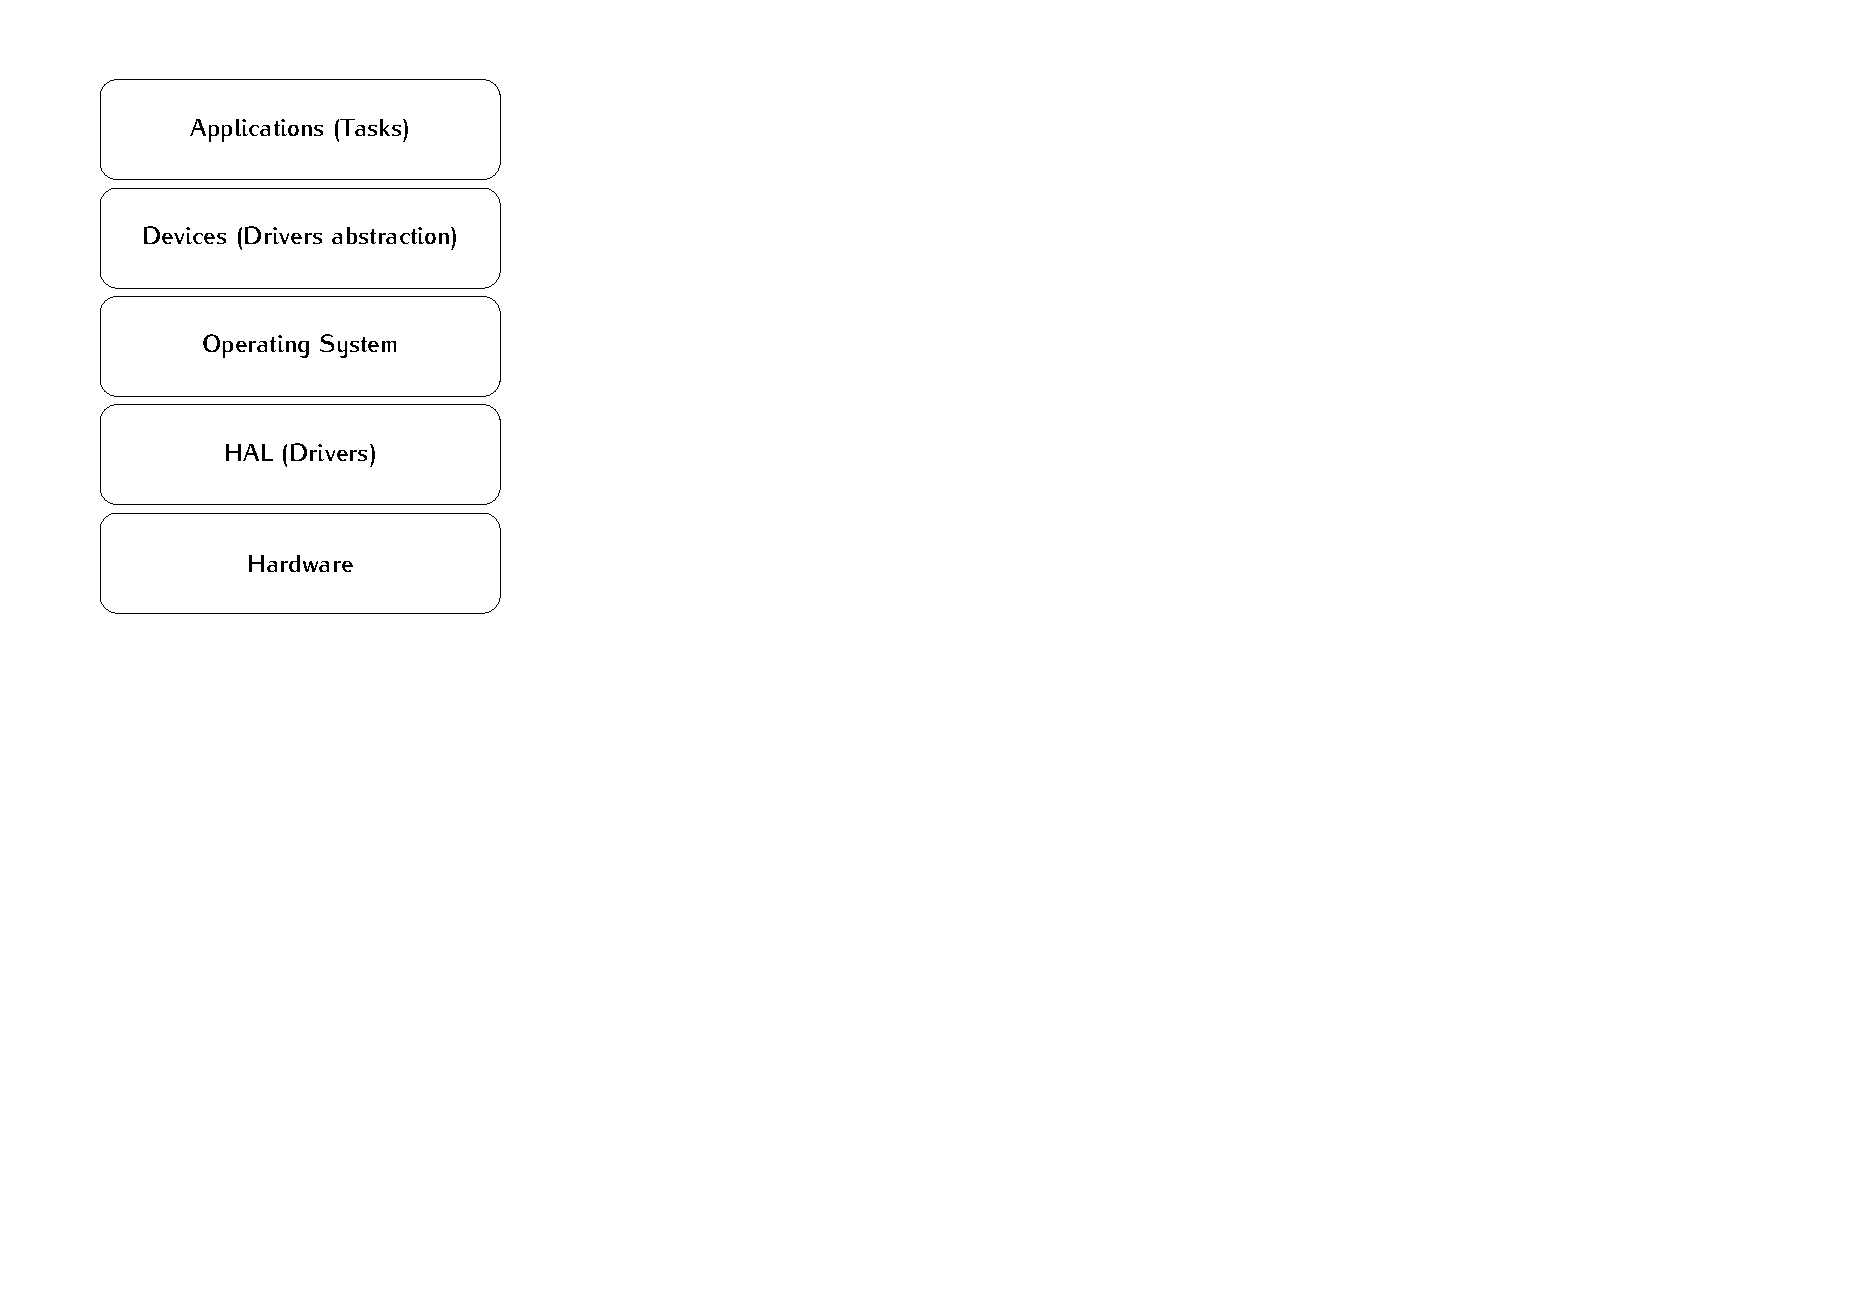
\includegraphics[width=0.4\textwidth]{figures/system_layers.pdf}
        \caption{System layers.}
        \label{fig:system-layers}
    \end{center}
\end{figure}

\section{Operation}

The system operates through the sequencial execution of routines (tasks in the context of the operating system) that are scheduled and multiplexed along the time. Each routine has a priority and a periodicity, which determine the following execution, the set of functionalities currentely running, and the memory usage management. Besides this deterministic scheduling system, the routines have communication channels with each other through the usage of queues, which provides a robust synchorization scheme. In the \autoref{ch:firmware} the system operation and the internal nuances are described in detail. Then, this section use a top view user perspective to describe the module operation.

\subsection{Execution Flow}
% Add here a diagram showing a simple flowchart or use cases to represent how the OBDH works.  

\subsection{Data Flow}
% Add here a flowchart or diagram showing where and how the data is generated and transfered across diferent modules and peripherals.

\subsection{Status LEDs} \label{sec:status-leds}

On the development version of the board, there are eight LEDs that indicates some behaviours of the systems. This set of LEDs can be seen on \autoref{fig:status-leds}.

\begin{figure}[!ht]
    \begin{center}
        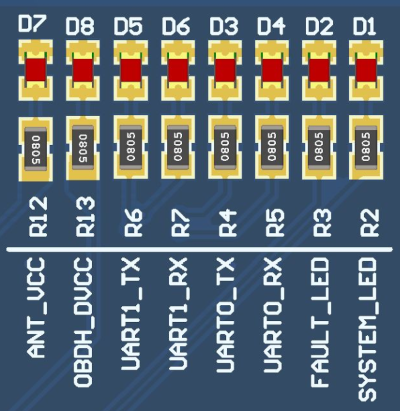
\includegraphics[width=0.3\textwidth]{figures/status_leds.png}
        \caption{Available status LEDs.}
        \label{fig:status-leds}
    \end{center}
\end{figure}

A description of each of these LED\nomenclature{\textbf{LED}}{\textit{Light-Emitting Diode.}}s are available below:

\begin{itemize}
    \item \textbf{D1 - System LED}: Heartbeat of the system. Blinks at a frequency of 1 Hz when the system is running properly.
    \item \textbf{D2 - Fault LED}: Indicates a critical fault in the system.
    \item \textbf{D3 - UART0 TX}: Blinks when data is being transmitted over the UART0 port.
    \item \textbf{D4 - UART0 RX}: Blinks when data is being received over the UART0 port.
    \item \textbf{D5 - UART1 TX}: Blinks when data is being transmitted over that UART1 port.
    \item \textbf{D6 - UART1 RX}: Blinks when data is being received over the UART1 port.
    \item \textbf{D7 - Antenna VCC}: Indicates that the antenna module board is being power sourced.
    \item \textbf{D8 - OBDH VCC}: Indicates that the OBDH board is being power sourced.
\end{itemize}

These LEDs are not mounted in the flight version of the module.
